\documentclass[tikz]{standalone}

\usepackage[T1]{fontenc}
\usepackage[english]{babel}

\usepackage{tikz}
\usetikzlibrary{calc}

\usepackage{pgfplots}


\begin{document}
	\begin{tikzpicture}
		\node (dsm) at (0,0) {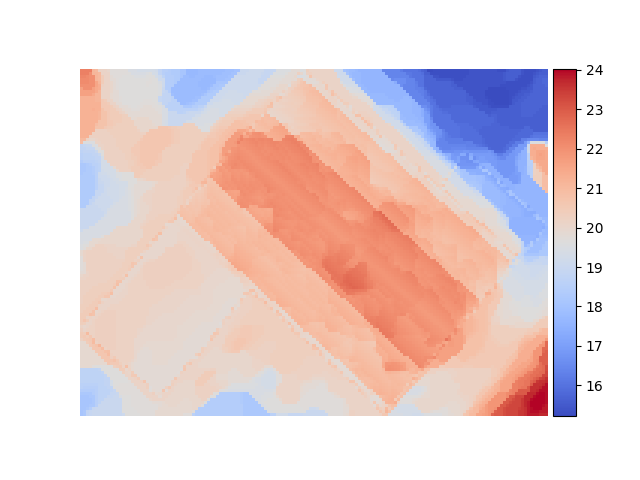
\includegraphics[height=3cm]{images/height_features/dsm-292034}};
        \path (dsm.south) + (0,-1.5) node[black] (dsm_2) {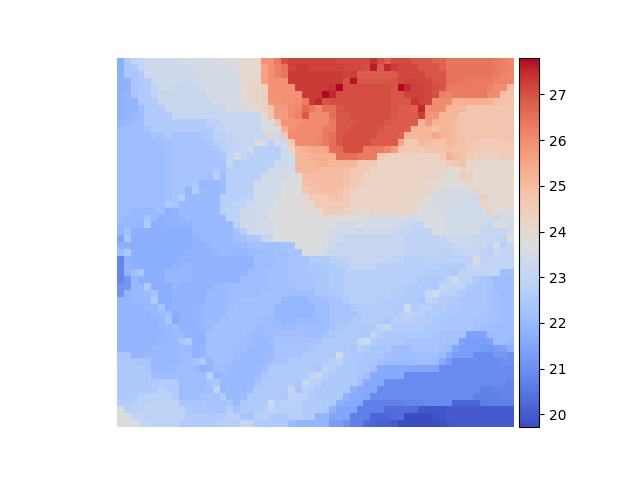
\includegraphics[height=3cm]{images/height_features/dsm-61215}};
        \path (dsm_2.south) + (0,-.25) node (dsm_legend) {(a) DSM};
        \path (dsm.east) + (2,0) node (simulated) {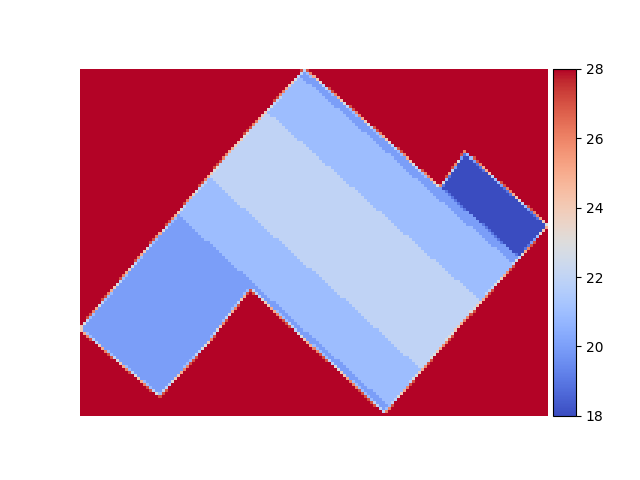
\includegraphics[height=3cm]{images/height_features/heightmap-292034}};
        \path (simulated.south) + (0,-1.5) node (simulated_2) {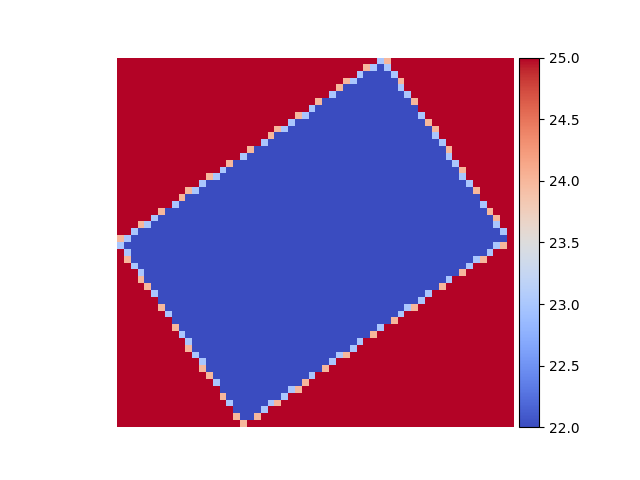
\includegraphics[height=3cm]{images/height_features/heightmap-61215}};
        \path (simulated_2.south) + (0,-.25) node (sim_legend) {(b) Model heightmap};
        \path (simulated.east) + (2,0) node (residual) {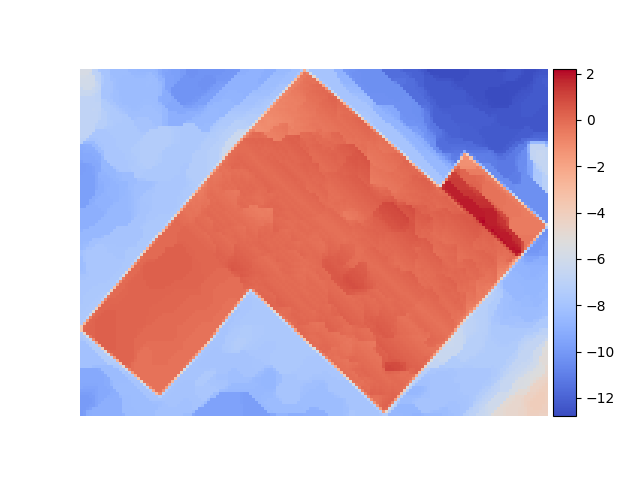
\includegraphics[height=3cm]{images/height_features/residual-292034}};
        \path (residual.south) + (0,-1.5) node (residual_2) {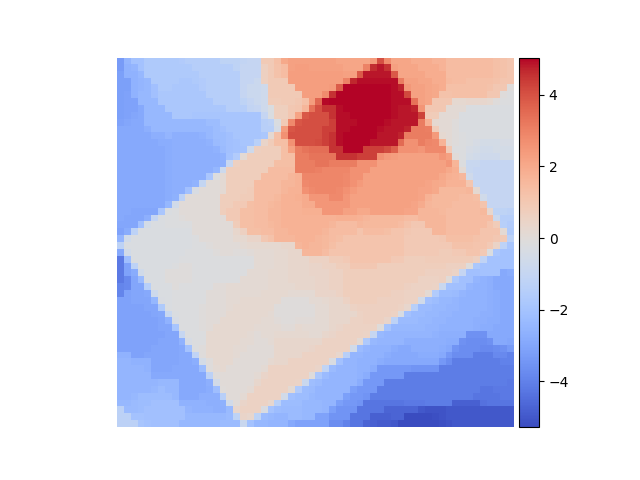
\includegraphics[height=3cm]{images/height_features/residual-61215}};
        \path (residual_2.south) + (0,-.25) node (res_legend) {(c) Residual};
        \path ($(dsm)!0.52!(simulated)$) node (minus) {\large --};
        \path ($(simulated)!0.51!(residual)$) node (equals) {\large =};
        \path ($(dsm)!0.52!(simulated)$) + (0, -3) node (minus) {\large --};
        \path ($(simulated)!0.51!(residual)$) + (0, -3) node (equals) {\large =};
        \path (residual) + (2, .17) node (top_dash_mapsto) {};
        \draw (residual) + (2, -.05) -- (top_dash_mapsto);
        \path (residual_2) + (2, .17) node (top_dash_mapsto_2) {};
        \draw (residual_2) + (2, -.05) -- (top_dash_mapsto_2);
        \path (residual) + (2.75,0) node (end_mapsto) {};
        \path (residual_2) + (2.75,0) node (end_mapsto_2) {};
        \draw[->] (residual) + (2,0) -- (end_mapsto) node[above, midway] {};
        \draw[->] (residual_2) + (2,0) -- (end_mapsto_2) node[above, midway] {};
        \path (end_mapsto) + (1, -1) node (hist) {};
        \path (end_mapsto_2) + (1, -1) node (hist_2) {};
        \path (hist.south |- dsm_legend) + (1.25, 0) node (hist_legend) {(d) Histogram};
        \begin{axis}[
            at={(hist)},
            width=4cm,
            height=4cm,
            area style,
        ]
            \addplot+[ybar interval,mark=no] plot coordinates {
                (-15, 0) 
                (-14, 0)
                (-13, 876)
                (-12, 366)
                (-11, 593)
                (-10, 675)
                (-9, 2231)
                (-8, 3623)
                (-7, 546)
                (-6, 159)
                (-5, 182)
                (-4, 70)
                (-3, 54)
                (-2, 123)
                (-1, 3815)
                (0, 4291)
                (1, 211)
                (2, 10)
                (3, 0)
                (4, 0)
                (5, 0)
                (6, 0)
                (7, 0)
                (8, 0)
            };
        \end{axis}
        \begin{axis}[
            at={(hist_2)},
            width=4cm,
            height=4cm,
            area style,
        ]
            \addplot+[ybar interval,mark=no] plot coordinates {
                (-15, 0)
                (-14, 0)
                (-13, 0)
                (-12, 0)
                (-11, 0)
                (-10, 0)
                (-9, 0)
                (-8, 0)
                (-7, 0)
                (-6, 17)
                (-5, 177)
                (-4, 143)
                (-3, 664)
                (-2, 219)
                (-1, 372)
                (0, 696)
                (1, 384)
                (2, 252)
                (3, 46)
                (4, 105)
                (5, 57)
                (6, 0)
                (7, 0)
                (8, 0)
            };
        \end{axis}
	\end{tikzpicture}
\end{document}
